\documentclass[aspectratio=169]{beamer}
\setbeamertemplate{footline}[frame number]
%\documentclass[aspectratio=169,notes=only]{beamer}
\usepackage{multicol}
\usepackage{wrapfig}
\usepackage{algorithmicx}
\usepackage{algpseudocode}
\usepackage{graphicx}
%\usepackage{subcaption} % cannot be used

\usepackage[english]{layout}
\usepackage[utf8]{inputenc}
\usepackage[english]{babel}
\usepackage[T1]{fontenc}
\usepackage{amsmath, soul, color, multicol, type1cm, verbatim, latexsym, dsfont, float, listings,alltt,tikz, lmodern, textcomp}
\usepackage[official]{eurosym}
\usepackage[export]{adjustbox}
\usepackage[caption = false]{subfig}
%\usepackage{beamerthemesplit}
%\usetheme{Frankfurt}
\usecolortheme{lily}
%\usefonttheme{structuresmallcapsserif}
\usefonttheme{professionalfonts}
\setbeamercovered{transparent}

\newcommand{\pluseq}{\mathrel{{+}{=}}}

%NeSI Colors <-------------------------------------------------------------------------------------
\usecolortheme{lily}
\usecolortheme[RGB={47, 68, 71}]{structure} 
\definecolor{nesidark}{HTML}{2F4447}
\definecolor{nesilight}{HTML}{CED9DF}
\definecolor{nesigrey}{gray}{0.7}
\definecolor{nesilightgrey}{gray}{0.98}
\definecolor{nesidarkgrey}{gray}{0.3}
\definecolor{nesiblue}{HTML}{2B9FC2}
\setbeamercolor{block title}{fg=black,bg=nesigrey}
\setbeamercolor{block body}{bg=nesilightgrey,fg=nesidarkgrey}
\setbeamercolor{block body alerted}{bg=white,fg=black}
\setbeamercolor{alerted text}{bg=white,fg=black}
\addtobeamertemplate{frametitle}{\vskip+1.2ex}{}
%NeSI Custom Code Hightlight <---------------------------------------------------------------------------------------
\lstdefinestyle{customcode}{
  belowcaptionskip=1\baselineskip,
  breaklines=true,
  xleftmargin=\parindent,
  showstringspaces=false,
  basicstyle=\ttfamily,
  keywordstyle=\bfseries\color{green!40!black},
  commentstyle=\itshape\color{purple!40!black},
  identifierstyle=\color{blue},
  stringstyle=\color{orange},
}
%NeSI Title <---------------------------------------------------------------------------------------
\setbeamerfont{title}{size=\huge}
\frenchspacing
\hyphenation{NeSI}
%NeSI Template parameters <-------------------------------------------------------------------------
\setbeamertemplate{blocks}[default]
\useinnertheme{circles}
\setbeamertemplate{title page}[default][center,rounded=false,shadow=false]
\newcommand\BackgroundPicture[1]{%
\setbeamertemplate{background}{%
\parbox[c][\paperheight]{\paperwidth}{%
\vfill \hfill \includegraphics[height=\paperheight]{#1}
\hfill \vfill
}}}

%\pagenumbering{arabic}

%Content Starts Here <-------------------------------------------------------------------------------
\title{\LARGE{Two interpolation methods for vector fields that conserve flux and line integrals}}
%\subtitle{Computational Science team}
\author{Alexander Pletzer (NeSI/NIWA), Wolfgang Hayek (NIWA/NeSI) and Samantha Adams (UK Met Office)\\
(alexander.pletzer@nesi.org.nz) \\
 C3DIS, Canberra\\
 7 May 2019  }
\date{}

\begin{document}
\BackgroundPicture{NeSI/title.png}
\begin{frame}[plain]
  \vspace{+1.0cm}
  \titlepage
\end{frame}

% This will generate the outline. If you have several topics, uncomment the multicols 
\BackgroundPicture{NeSI/blank-01.png}

%%%%%%%%%%%%%%%%%%%%%%%%%%%%%%%%%%%%%%%%%%%%%%%%%%%%%%%%%%%%%%%%%%%%%%%%%%%%%%%%%%%%%%%%%%%%%%%
%%%%%%%%%%%%%%%%%%%%%%%%%%%%%%%%%%%%%%%% Some Examples %%%%%%%%%%%%%%%%%%%%%%%%%%%%%%%%%%%%%%%%
%%%%%%%%%%%%%%%%%%%%%%%%%%%%%%%%%%%%%%%%%%%%%%%%%%%%%%%%%%%%%%%%%%%%%%%%%%%%%%%%%%%%%%%%%%%%%%%
% List with bullets (itemize) <---
% The [<+-| alert@+>] will create a new slide for each element with highlighting 


\begin{frame}[t]
  \frametitle{Motivation: want answers to}
    \begin{block}{How to interpolate vector fields with staggered components?}
      \begin{itemize}%[<+-| alert@+>]
	  \item Arakawa C/D grids
      \item Components are on cell faces or edges
      \item Arises in computational fluid dynamics and electromagnetics
    \end{itemize}
  \end{block}
  \begin{tabular}{lr}
      % after \\: \hline or \cline{col1-col2} \cline{col3-col4} ...
      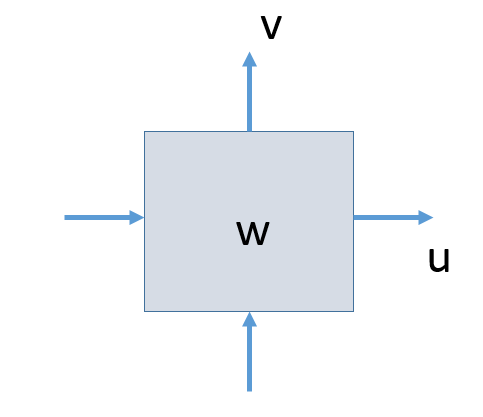
\includegraphics[width=30mm]{uvArakawaC.PNG} &               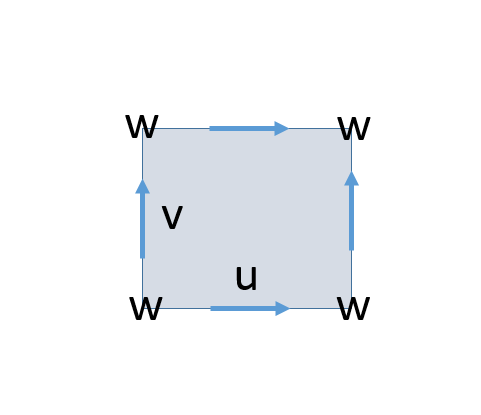
\includegraphics[width=30mm]{uvArakawaD.PNG} \\
      {Arakawa C-grid} & {Arakawa D-grid}  
\end{tabular}
\end{frame}

\begin{frame}[t]
  \frametitle{Currently used interpolation methods in earth sciences}
    \begin{block}{Is there hope to unify these?}
      \begin{itemize}%[<+-| alert@+>]
	  \item Linear
      \item Conservative or area weighted, used in climate studies to enforce conservation of total mass, energy
    \end{itemize}
  \end{block}
  \begin{tabular}{lcr}
      % after \\: \hline or \cline{col1-col2} \cline{col3-col4} ...
      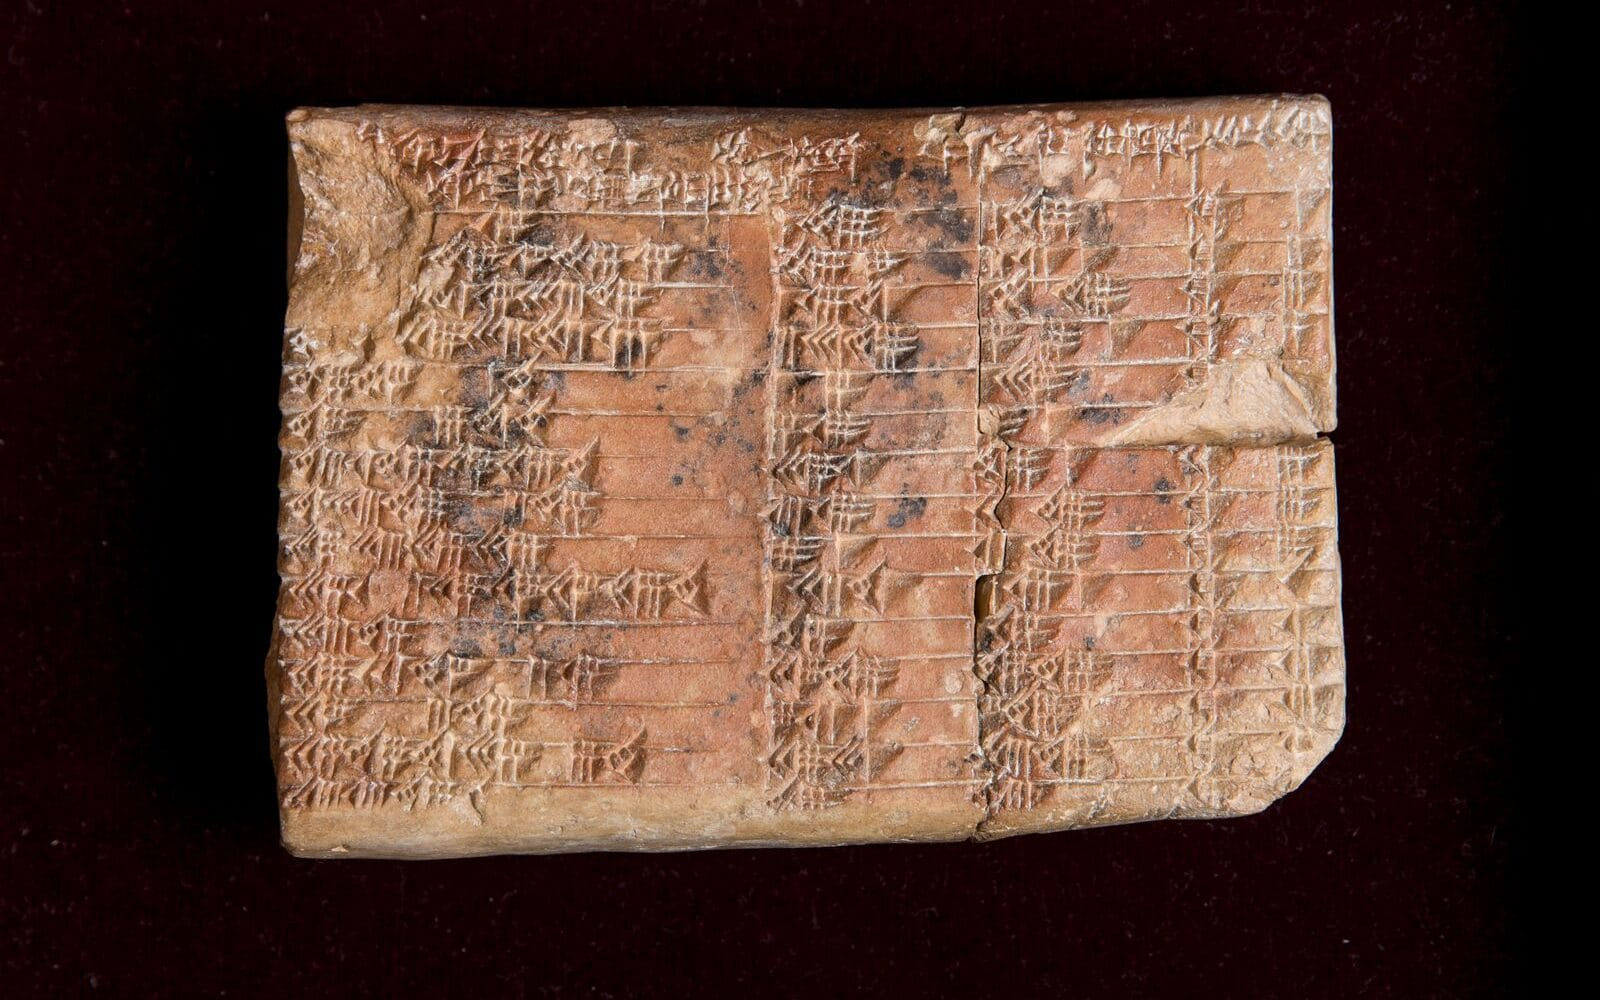
\includegraphics[width=30mm]{babylonianTablet.jpeg} & 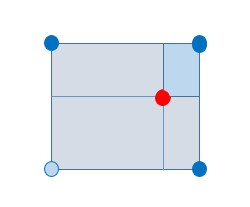
\includegraphics[width=30mm]{bilinear.png} & 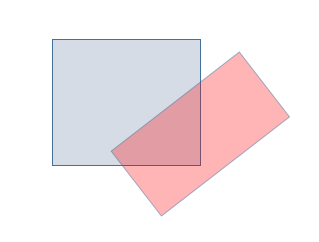
\includegraphics[width=30mm]{conservative.png} \\
      {Babylonian tablet (1700BC)} & {Bilinear} & {Conservative (used since the 1990s)}  
\end{tabular}
\end{frame}

\begin{frame}[t]
  \frametitle{Earth science grids are curvilinear}
  \begin{block}{Example: cubed-sphere grid employed by exascale weather prediction/climate modelling system LFRic developed at UK Met Office}
    \begin{itemize}
      \item Six logically rectangular grids (cannot be represented as a single structured grid)
      \item No pole-like singularity but some distortion where three tiles meet 
    \end{itemize}
  \end{block}
  \begin{center}
    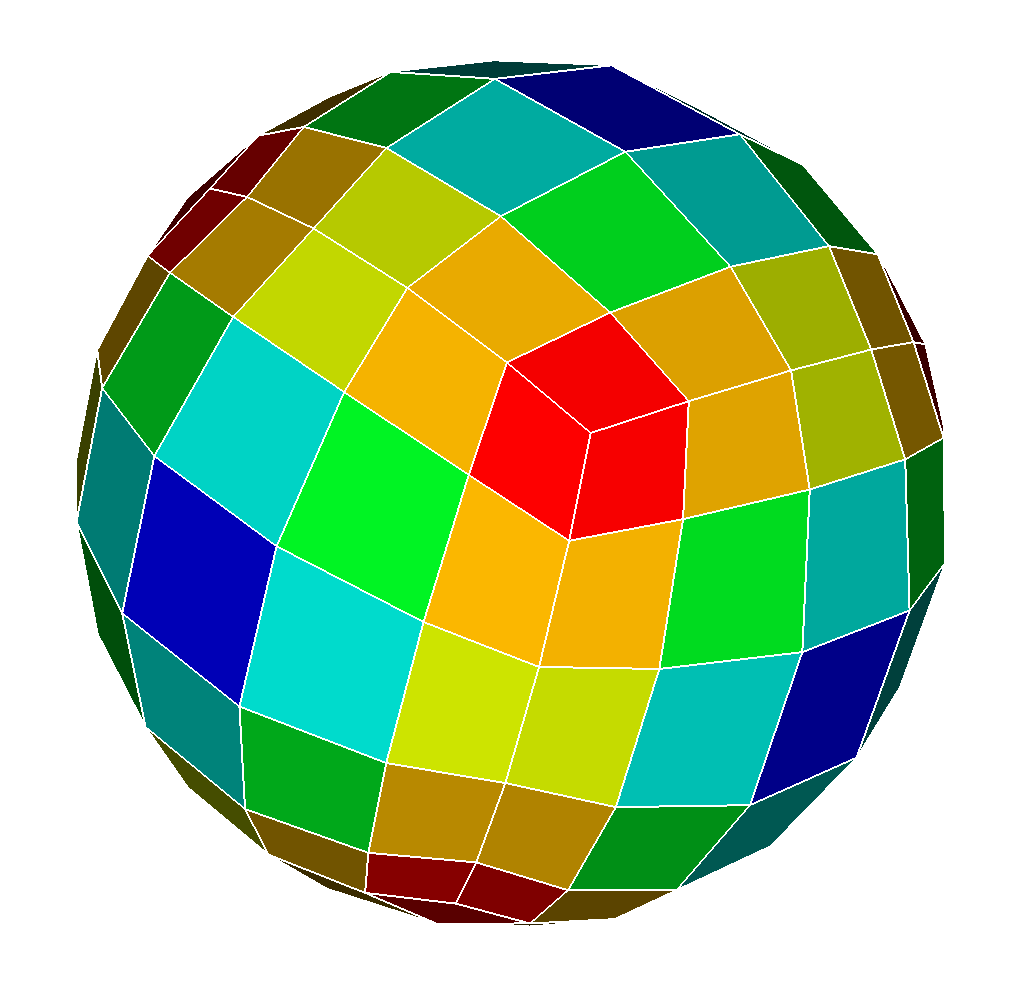
\includegraphics[width=0.35\textwidth]{cubedSphere.png}
  \end{center}
\end{frame}

\begin{frame}[t]
  \frametitle{Interpolation is required for}
  \begin{itemize}
   \item regridding/remapping fields deom one grid to another
   \item computing fluxes across an area
   \item advecting fields
   \item visualising streamlines
  \end{itemize}
    \begin{tabular}{lr}
      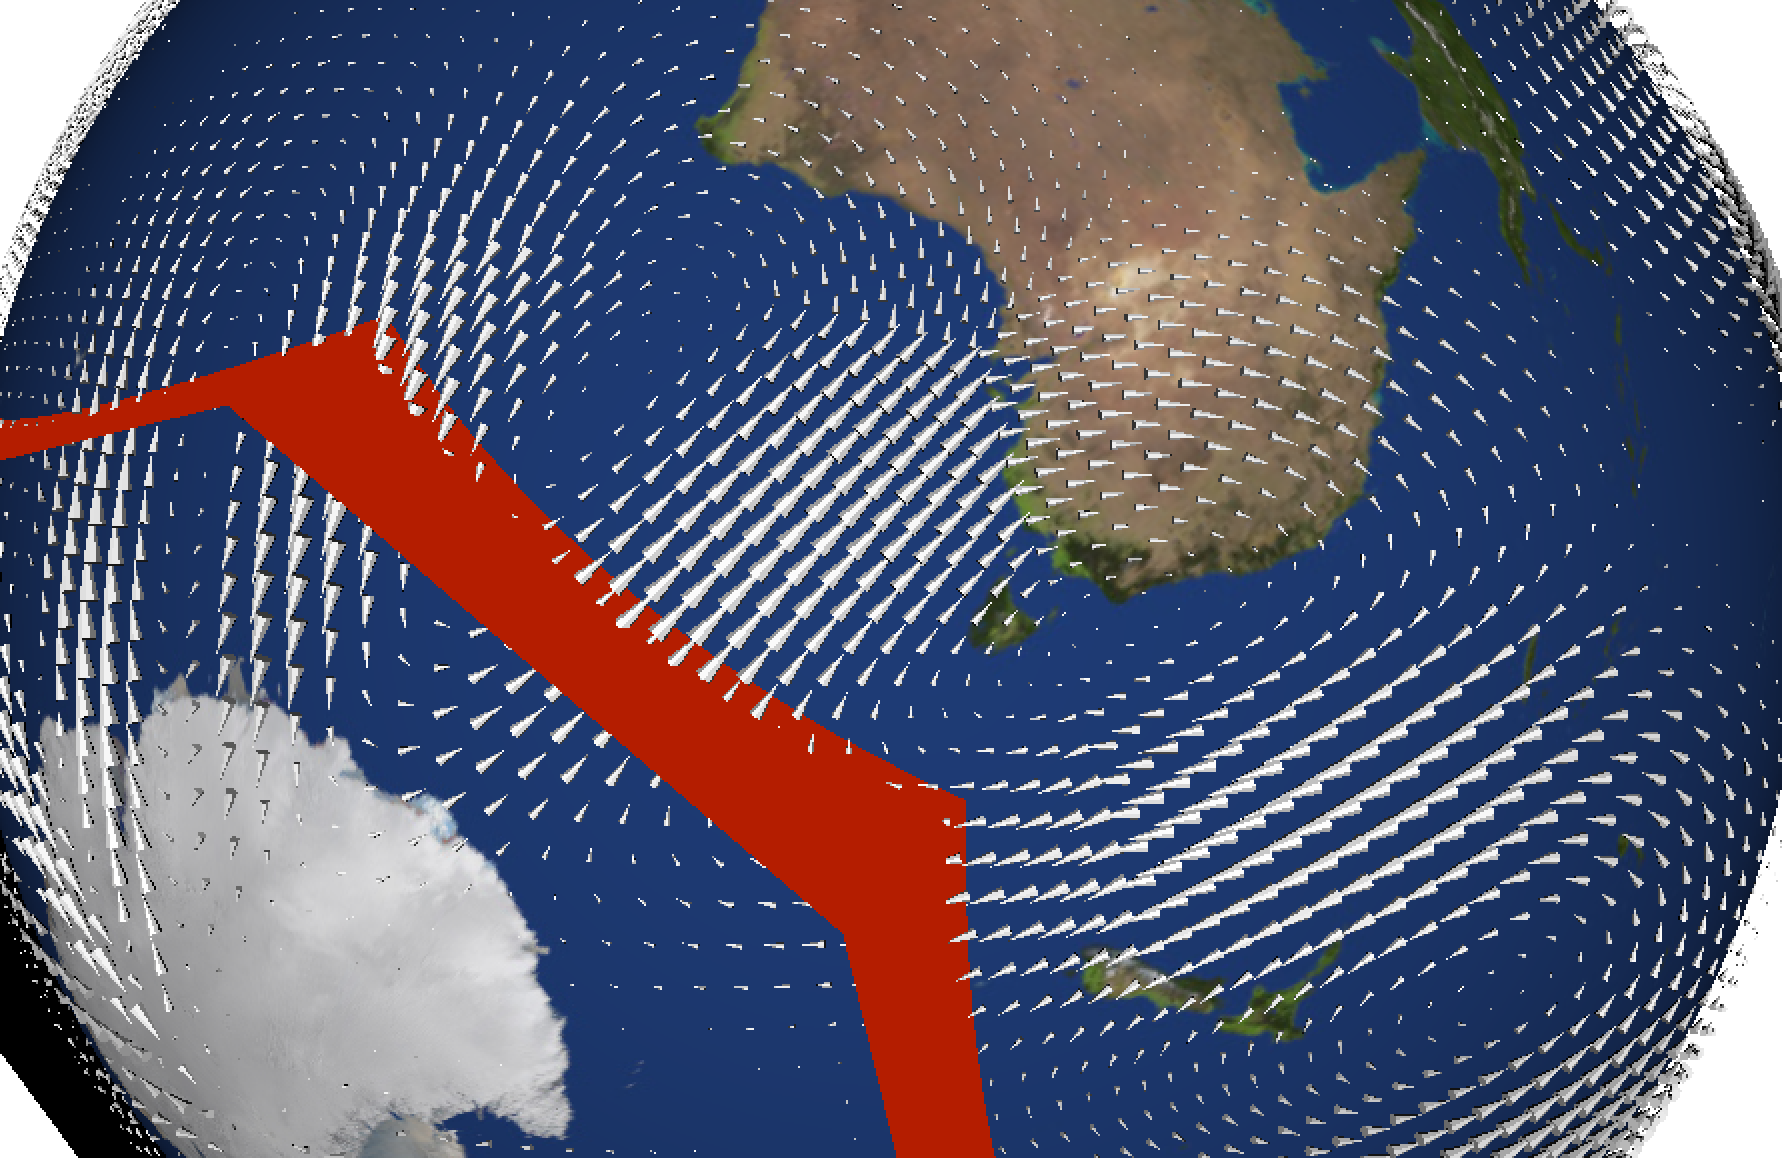
\includegraphics[width=40mm]{fluxIntegral.png} & 
      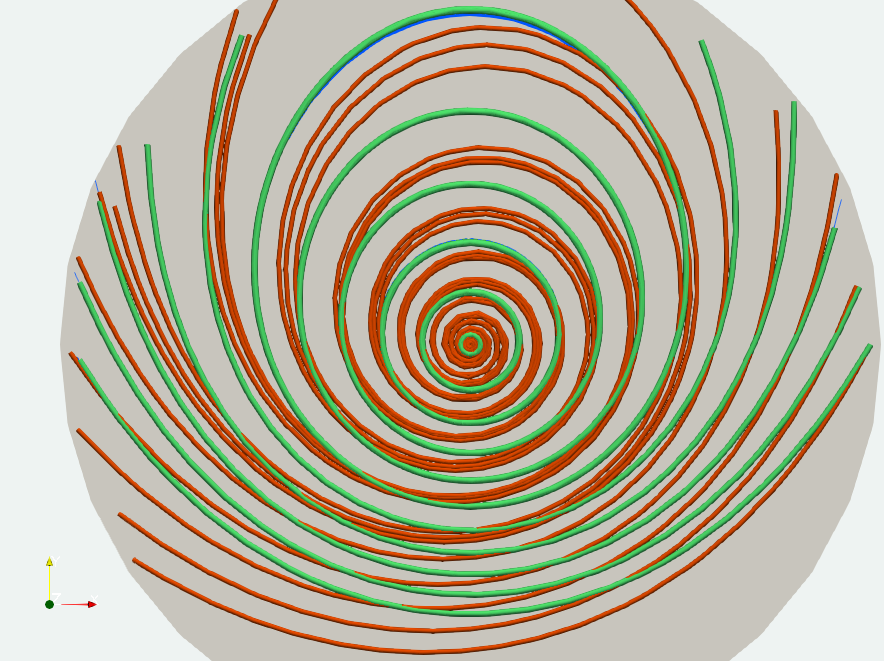
\includegraphics[width=40mm]{streamLineError.png} 
    \end{tabular}  
\end{frame}

\begin{frame}[t]
  \frametitle{Four types of fields - four types of interpolation methods}
  \begin{block}{Type of field determines staggering and interpolation method}
  \begin{itemize}
  	\item``Correct'' discretisation ensures that mimetic properties such as $\nabla \times \nabla = \nabla \cdot \nabla \times = 0$ are satisfied
  	\item ``Correct'' interpolation ensures conservation of line, surface and volume integrals (as appropriate)
  \end{itemize}
\end{block}
\begin{tabular} {|r|c|c|c|c|l|}
\hline
{\color{blue} field type}                 &  num.comp. & example         & staggering       & target  & {\color{blue} method}  \\
\hline
{\color{blue} scalar}                     &       1         & temperature     & nodal            &   point  & {\color{blue} bilinear} \\
{\color{magenta} vector}        &       {\color{red} 3}         & {\color{red} velocity}        & {\color{red} edges/Arakawa D} &  {\color{red} line}    & {\color{magenta} this talk} \\
{\color{magenta} pseudo-vector} &       {\color{red} 3}         & {\color{red} magnetic field}  & {\color{red} faces/Arakawa C}  &  {\color{red} surface} & {\color{magenta} this talk} \\
{\color{blue} pseudo-scalar}              &       1         & mass density    & cell centred     &  volume  & {\color{blue} conservative} \\
\hline
\end{tabular}

\end{frame}

\begin{frame}[fragile]{Generalizing ``interpolation'' to work for nodal, edge, face and cell fields}
\begin{block}{One formula for all cases}
$\int f = \sum_i {\color{cyan} f_i} \int_{\color{red} T} {\color{blue} \phi_i}$
\begin{itemize}
\item {\color{blue} $\phi_i$} is \textbf{basis} $k$-form, $k =$ 0, 1, 2 or 3
\item {\color{red} $T$} is \textbf{target} (point, line, area or volume)
\item ${\color{cyan} f_i}$ is \textbf{field integral} over cell element $k$ (node, edge, face or cell)
\item $\int_T \phi_i \equiv$ \textbf{interpolation weight}
\item $i$ index runs over all the degrees of freedom (points, edges, faces etc., as appropriate)
\end{itemize}
\end{block}
\end{frame}

\begin{frame}[fragile]{Basis functions $\phi_j$ satisfy orthogonality condition}

\begin{block}{$\int_i \phi_j = \delta_{ij}$}
   $i$ is cell element (node, edge, face, cell), $j$ is basis function index
 \end{block}
  \begin{tabular}{lr}
      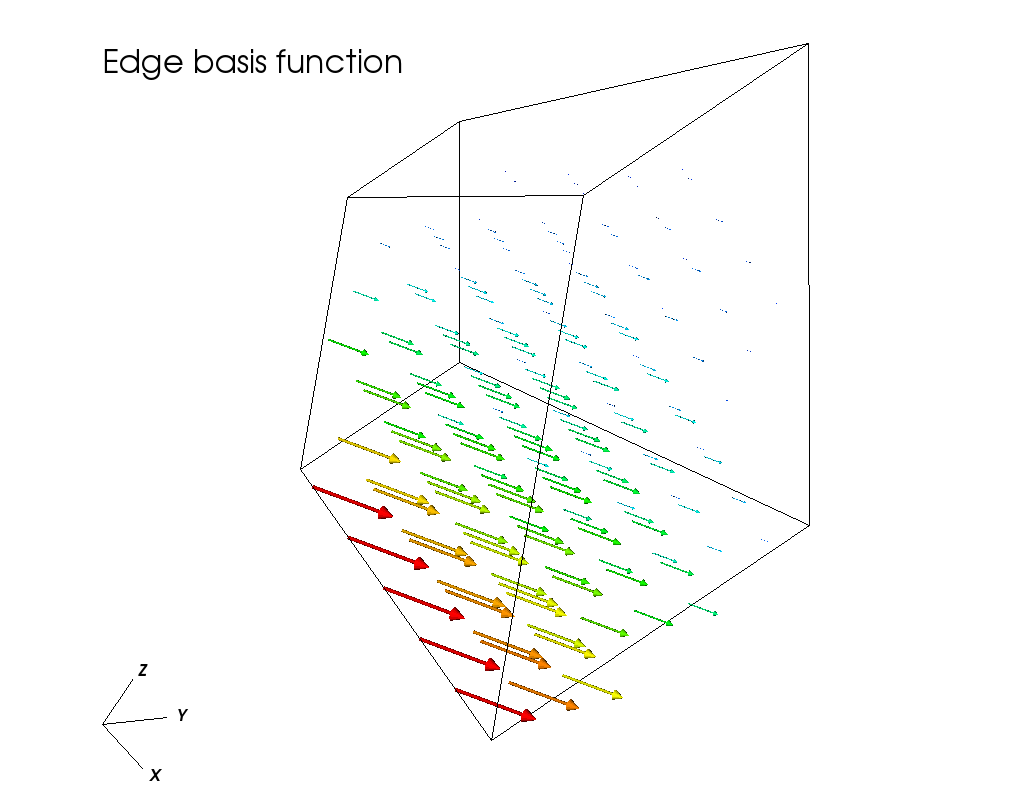
\includegraphics[width=50mm]{hexEdge.png} &                        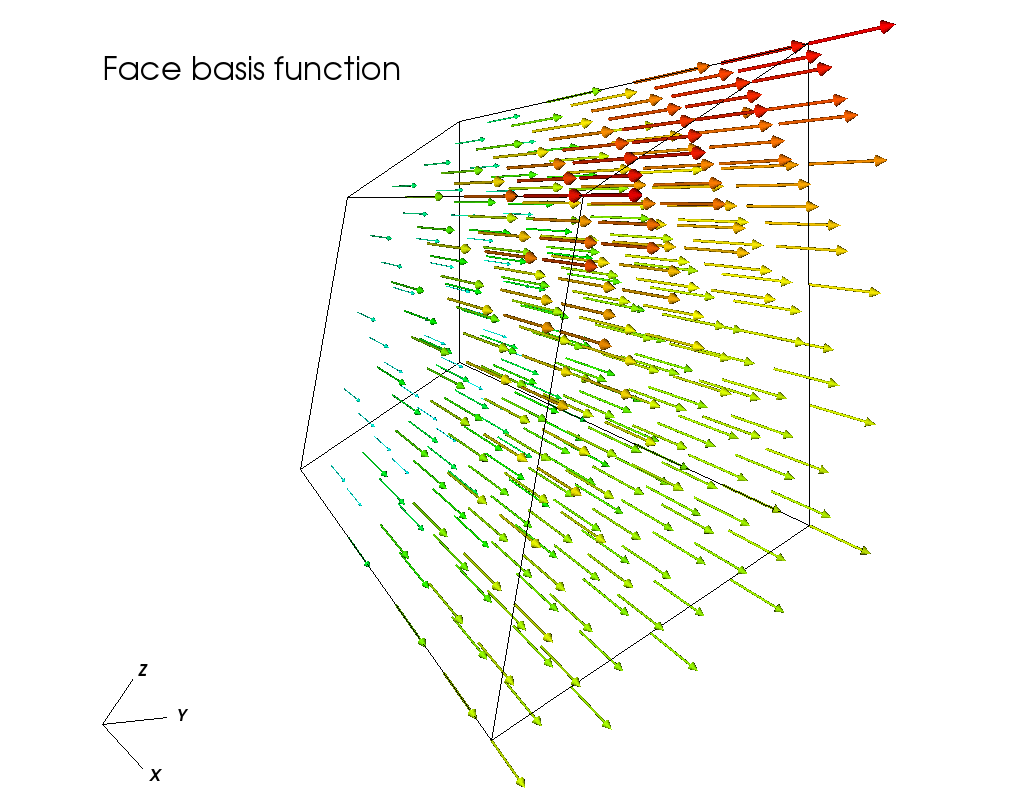
\includegraphics[width=50mm]{hexFace.png} \\
      {Edge basis is perpendicular } & {Face basis is tangent }  \\
      {to neighbouring edges} & {to neighbouring faces}
\end{tabular}

\end{frame}

\begin{frame}[t]
  \frametitle{Result 1: divergence-free field  $v = dz \wedge d\psi$}
  \begin{block}{Flux integral depends only on distance of endpoints to nearest grid node}
  \end{block}
  \begin{tabular}{c}
    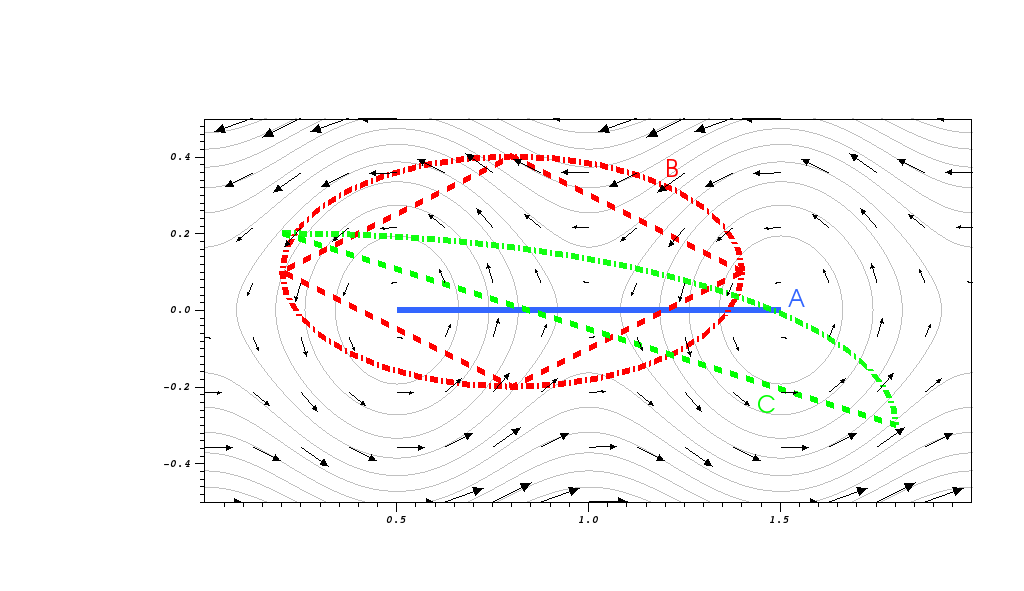
\includegraphics[width=.7\linewidth]{flow.png} \\
    Closed loop integral is exact!
  \end{tabular}
\end{frame}

\begin{frame}[t]
  \frametitle{Result 2: Singular, polar vector field $v = \frac{x dx + y dy}{2 \pi (x^2 + y^2)}$}
  \begin{block}{Loop integral is 1 if singularity is inside contour, 0 otherwise. Getting exact 0 for $E0$ and $E1$, exact 1 for $E6$-$E9$ and in between values for contours that intersect the cell containing (0,0)}
  \end{block}
  \begin{tabular}{lr}
  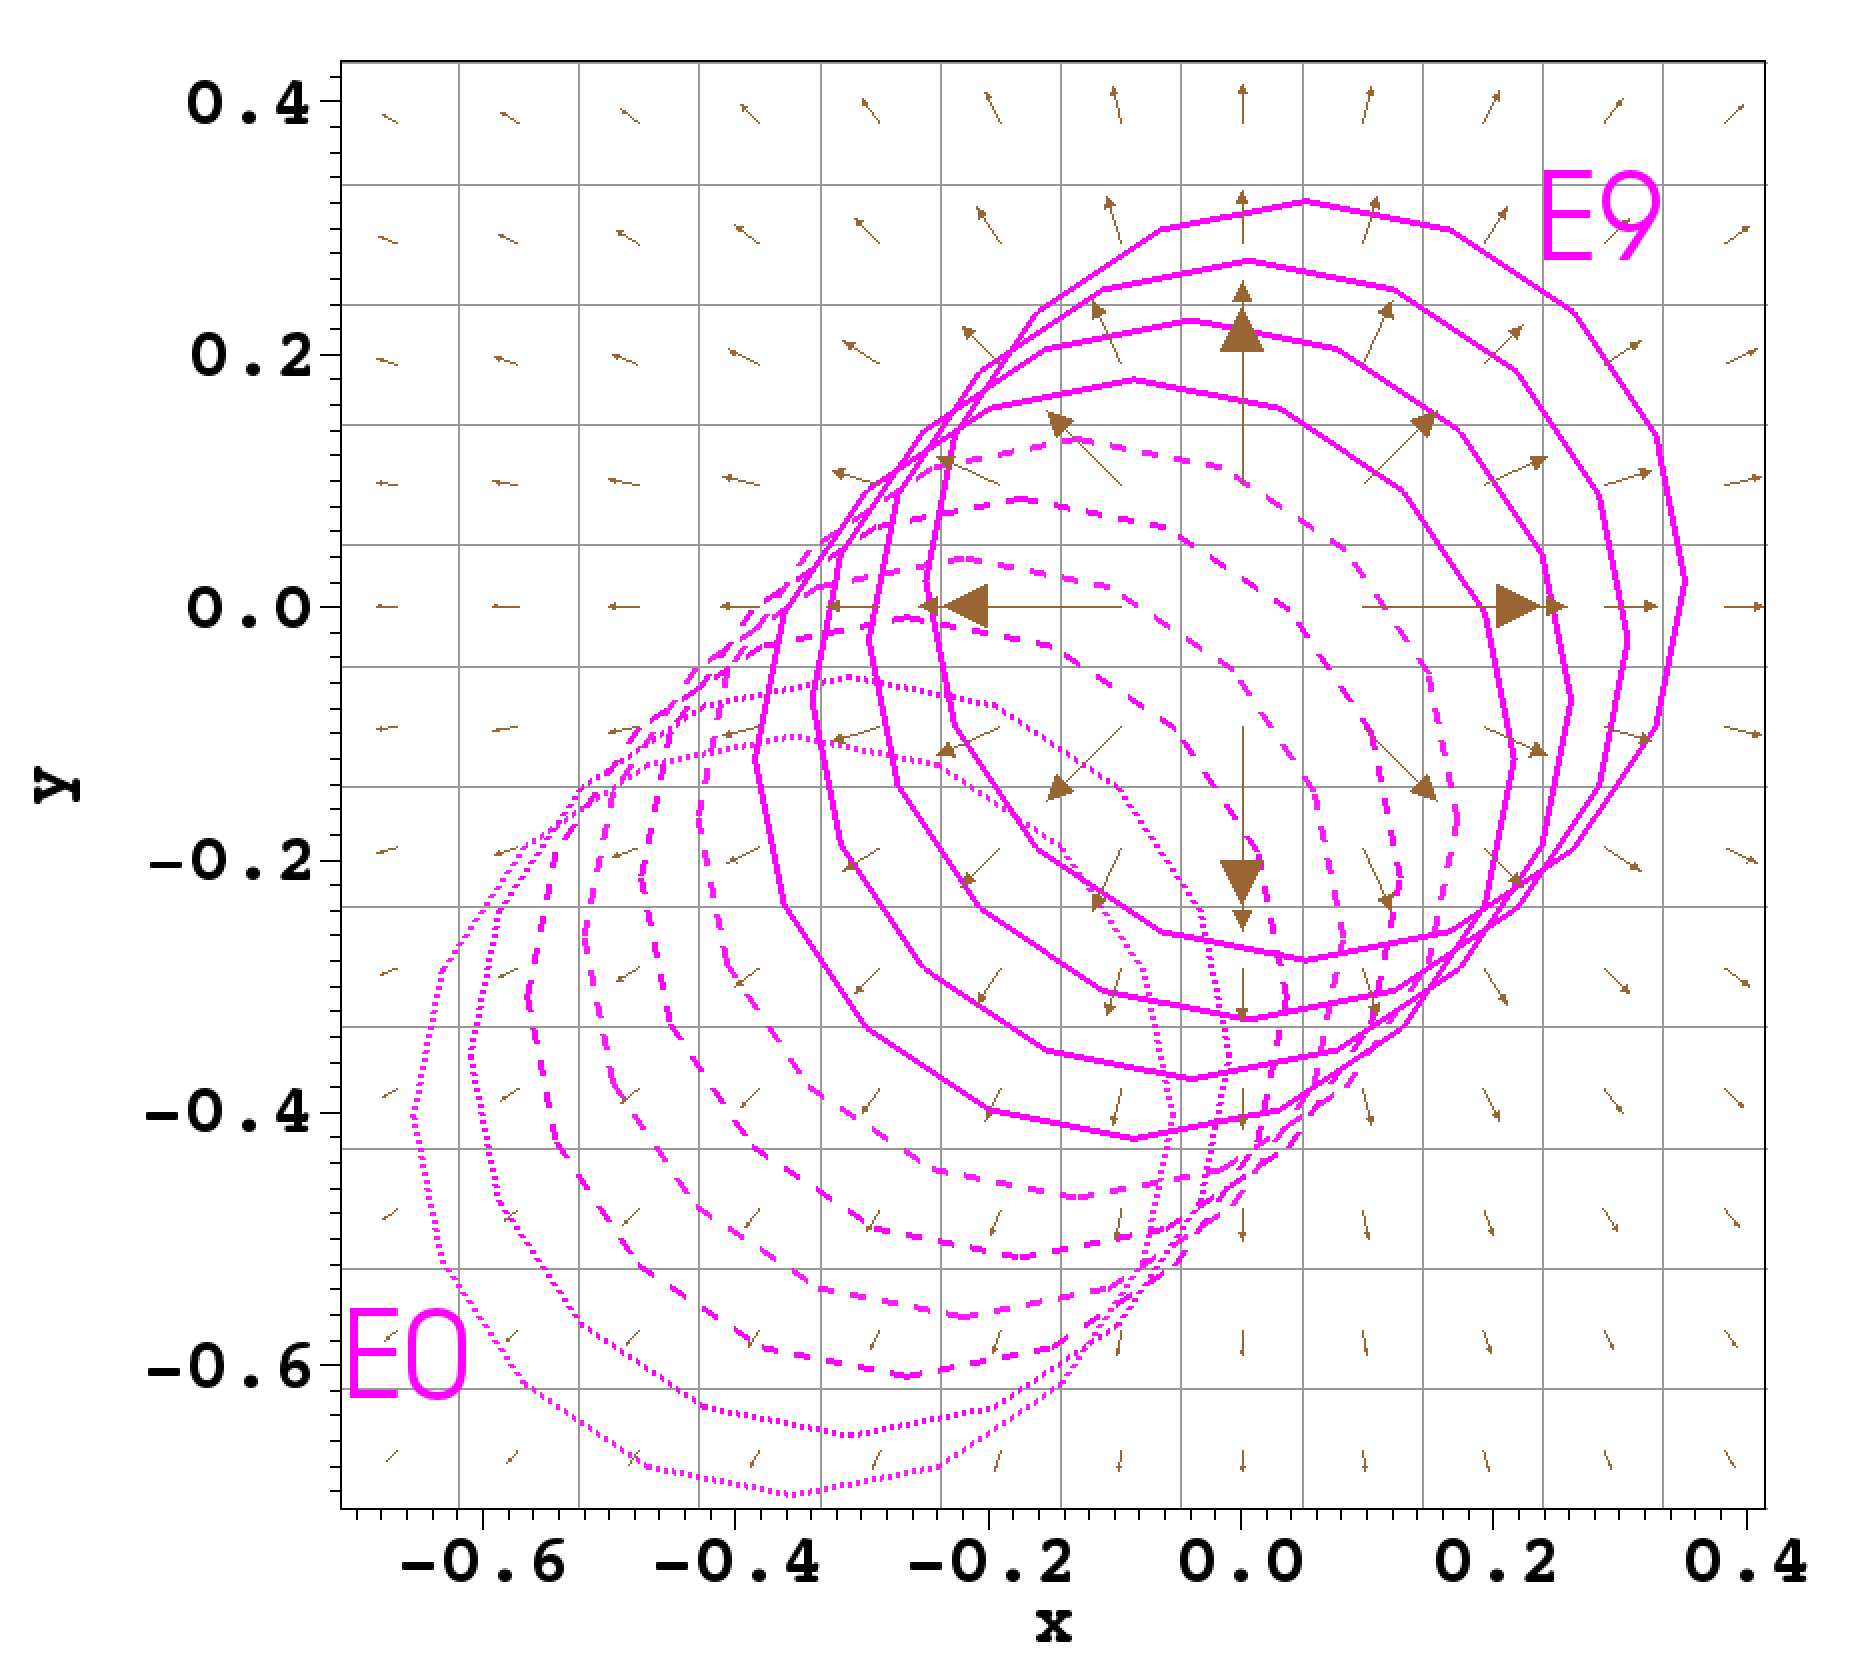
\includegraphics[width=50mm]{polar.png} & 
  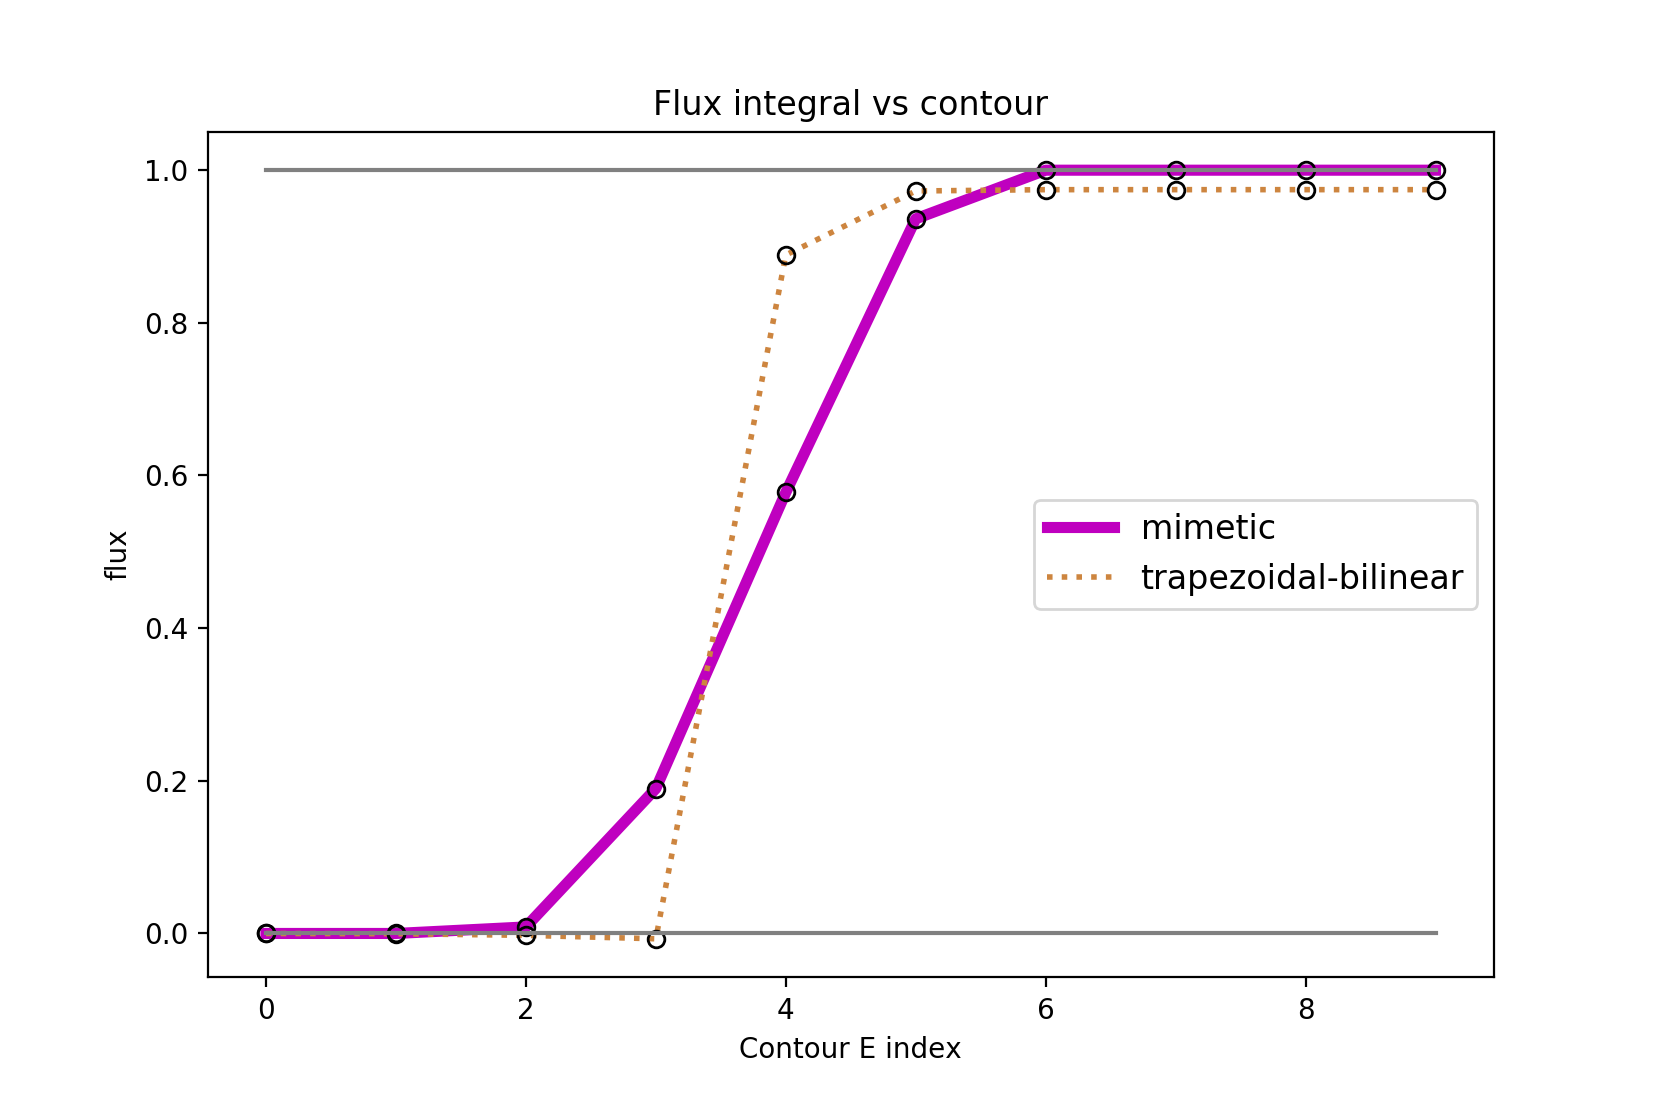
\includegraphics[width=80mm]{polarFluxes.png}
  \end{tabular}



  \begin{center}
    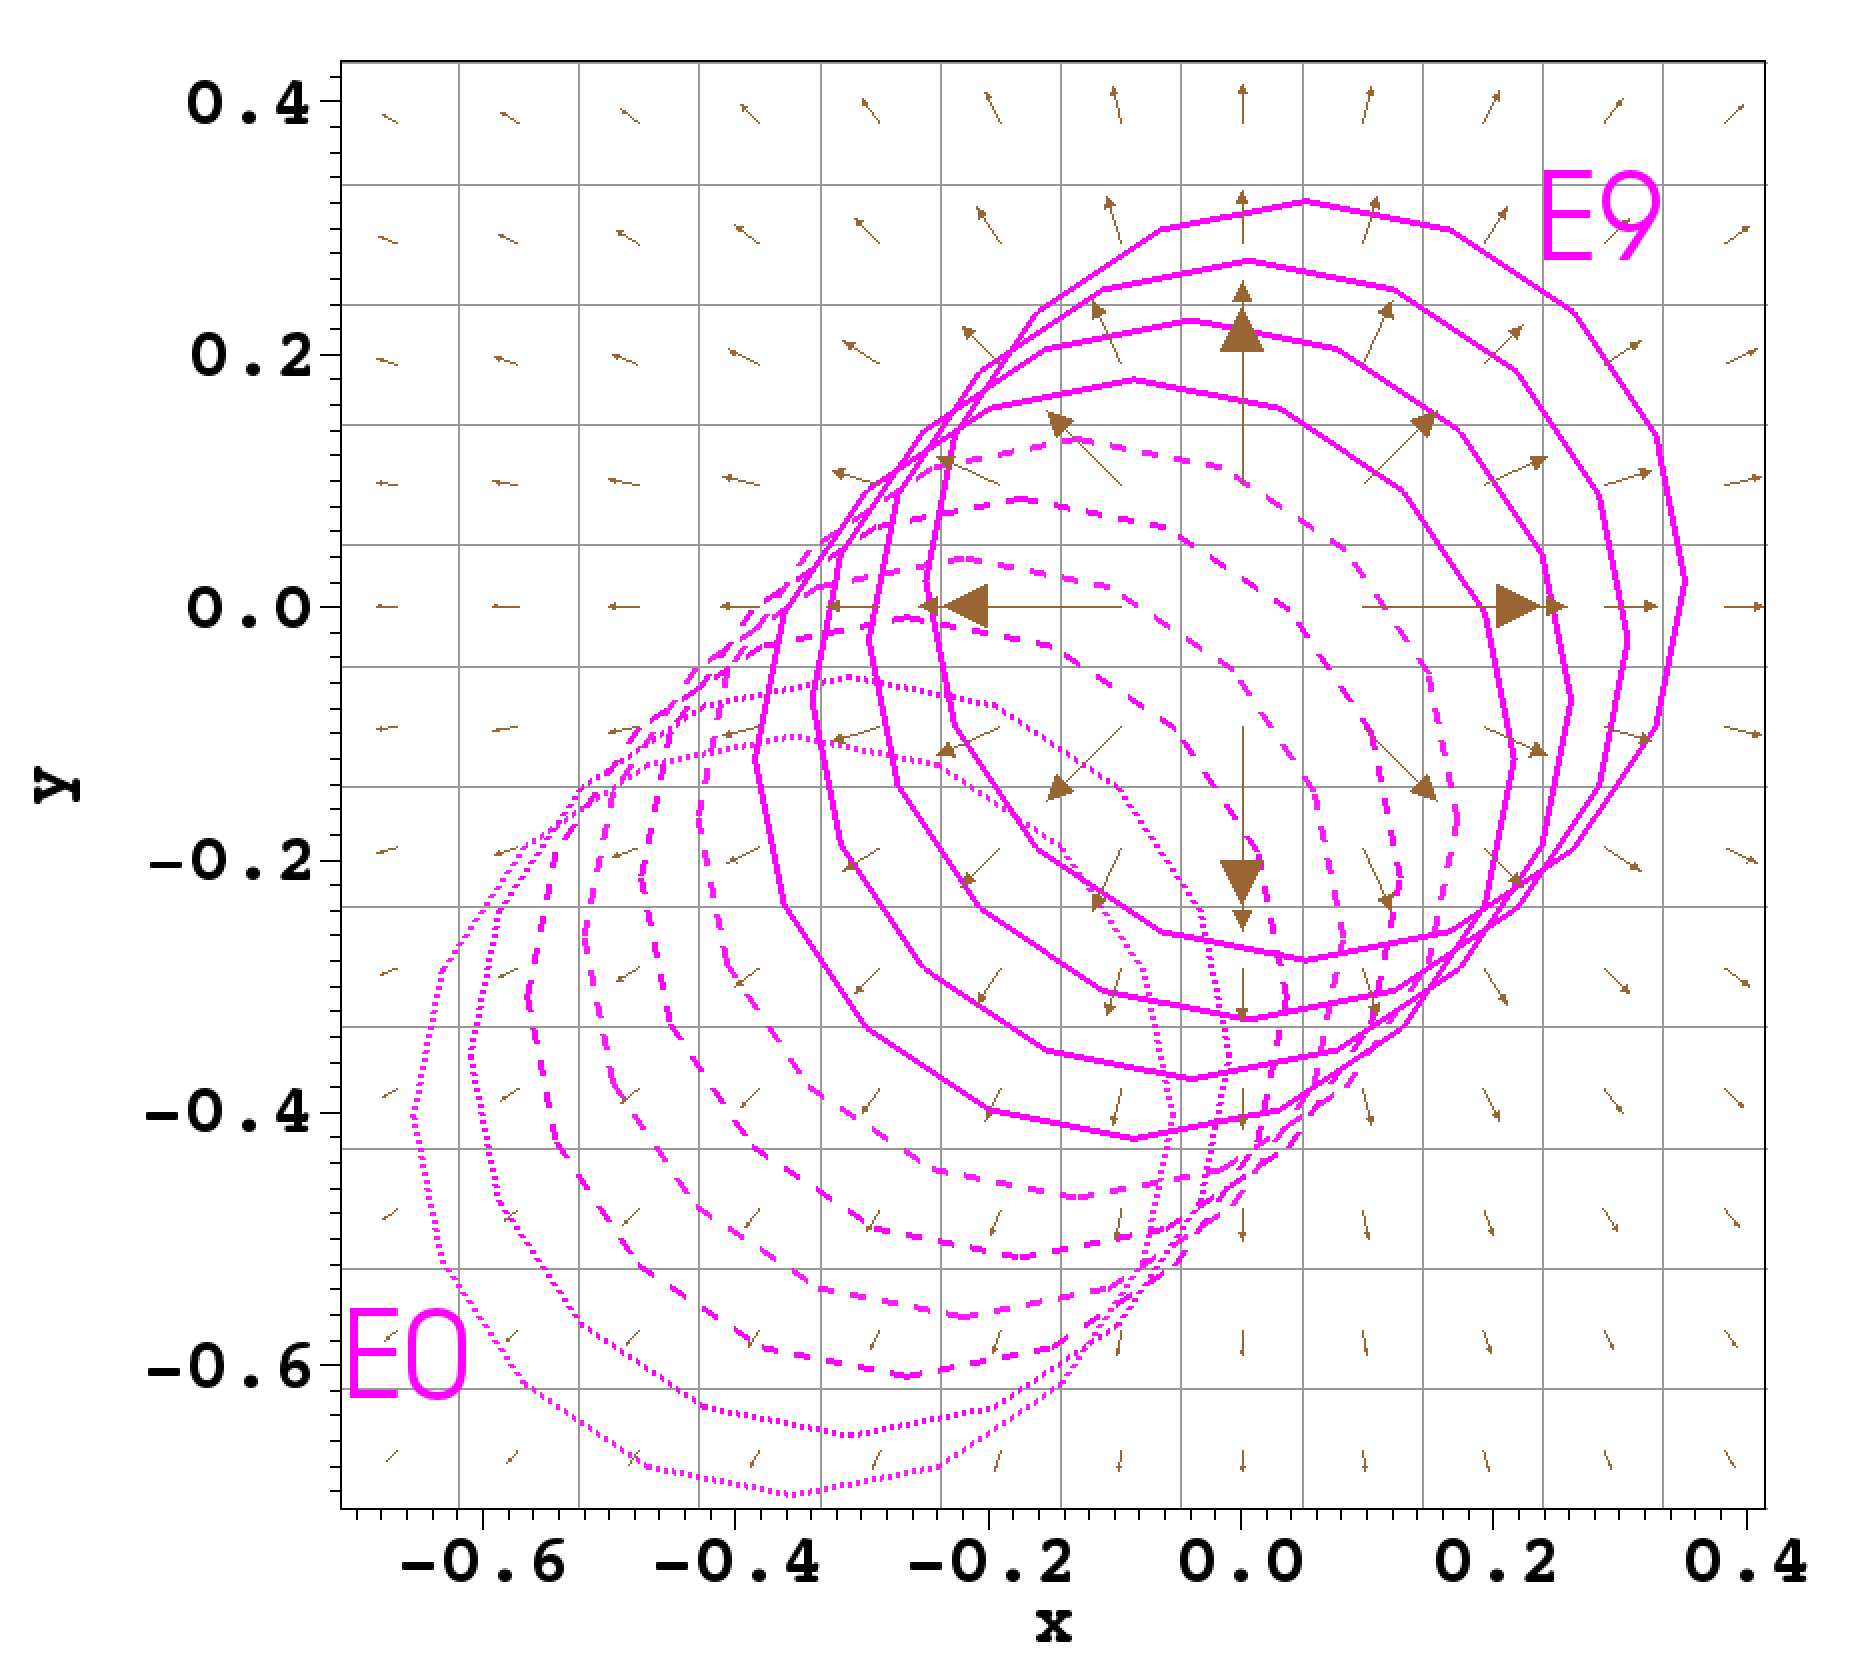
\includegraphics[width=.5\linewidth]{polar.png}
  \end{center}
\end{frame}

\begin{frame}[t]
  \frametitle{Result 3: flux on the cubed sphere $v = d\psi \wedge dr$}
  \begin{block}{Edge/face interpolation works for highly distorted cells. Zero error start/end points fall onto grid nodes.}
  \end{block}
  
  \begin{tabular}{lr}
  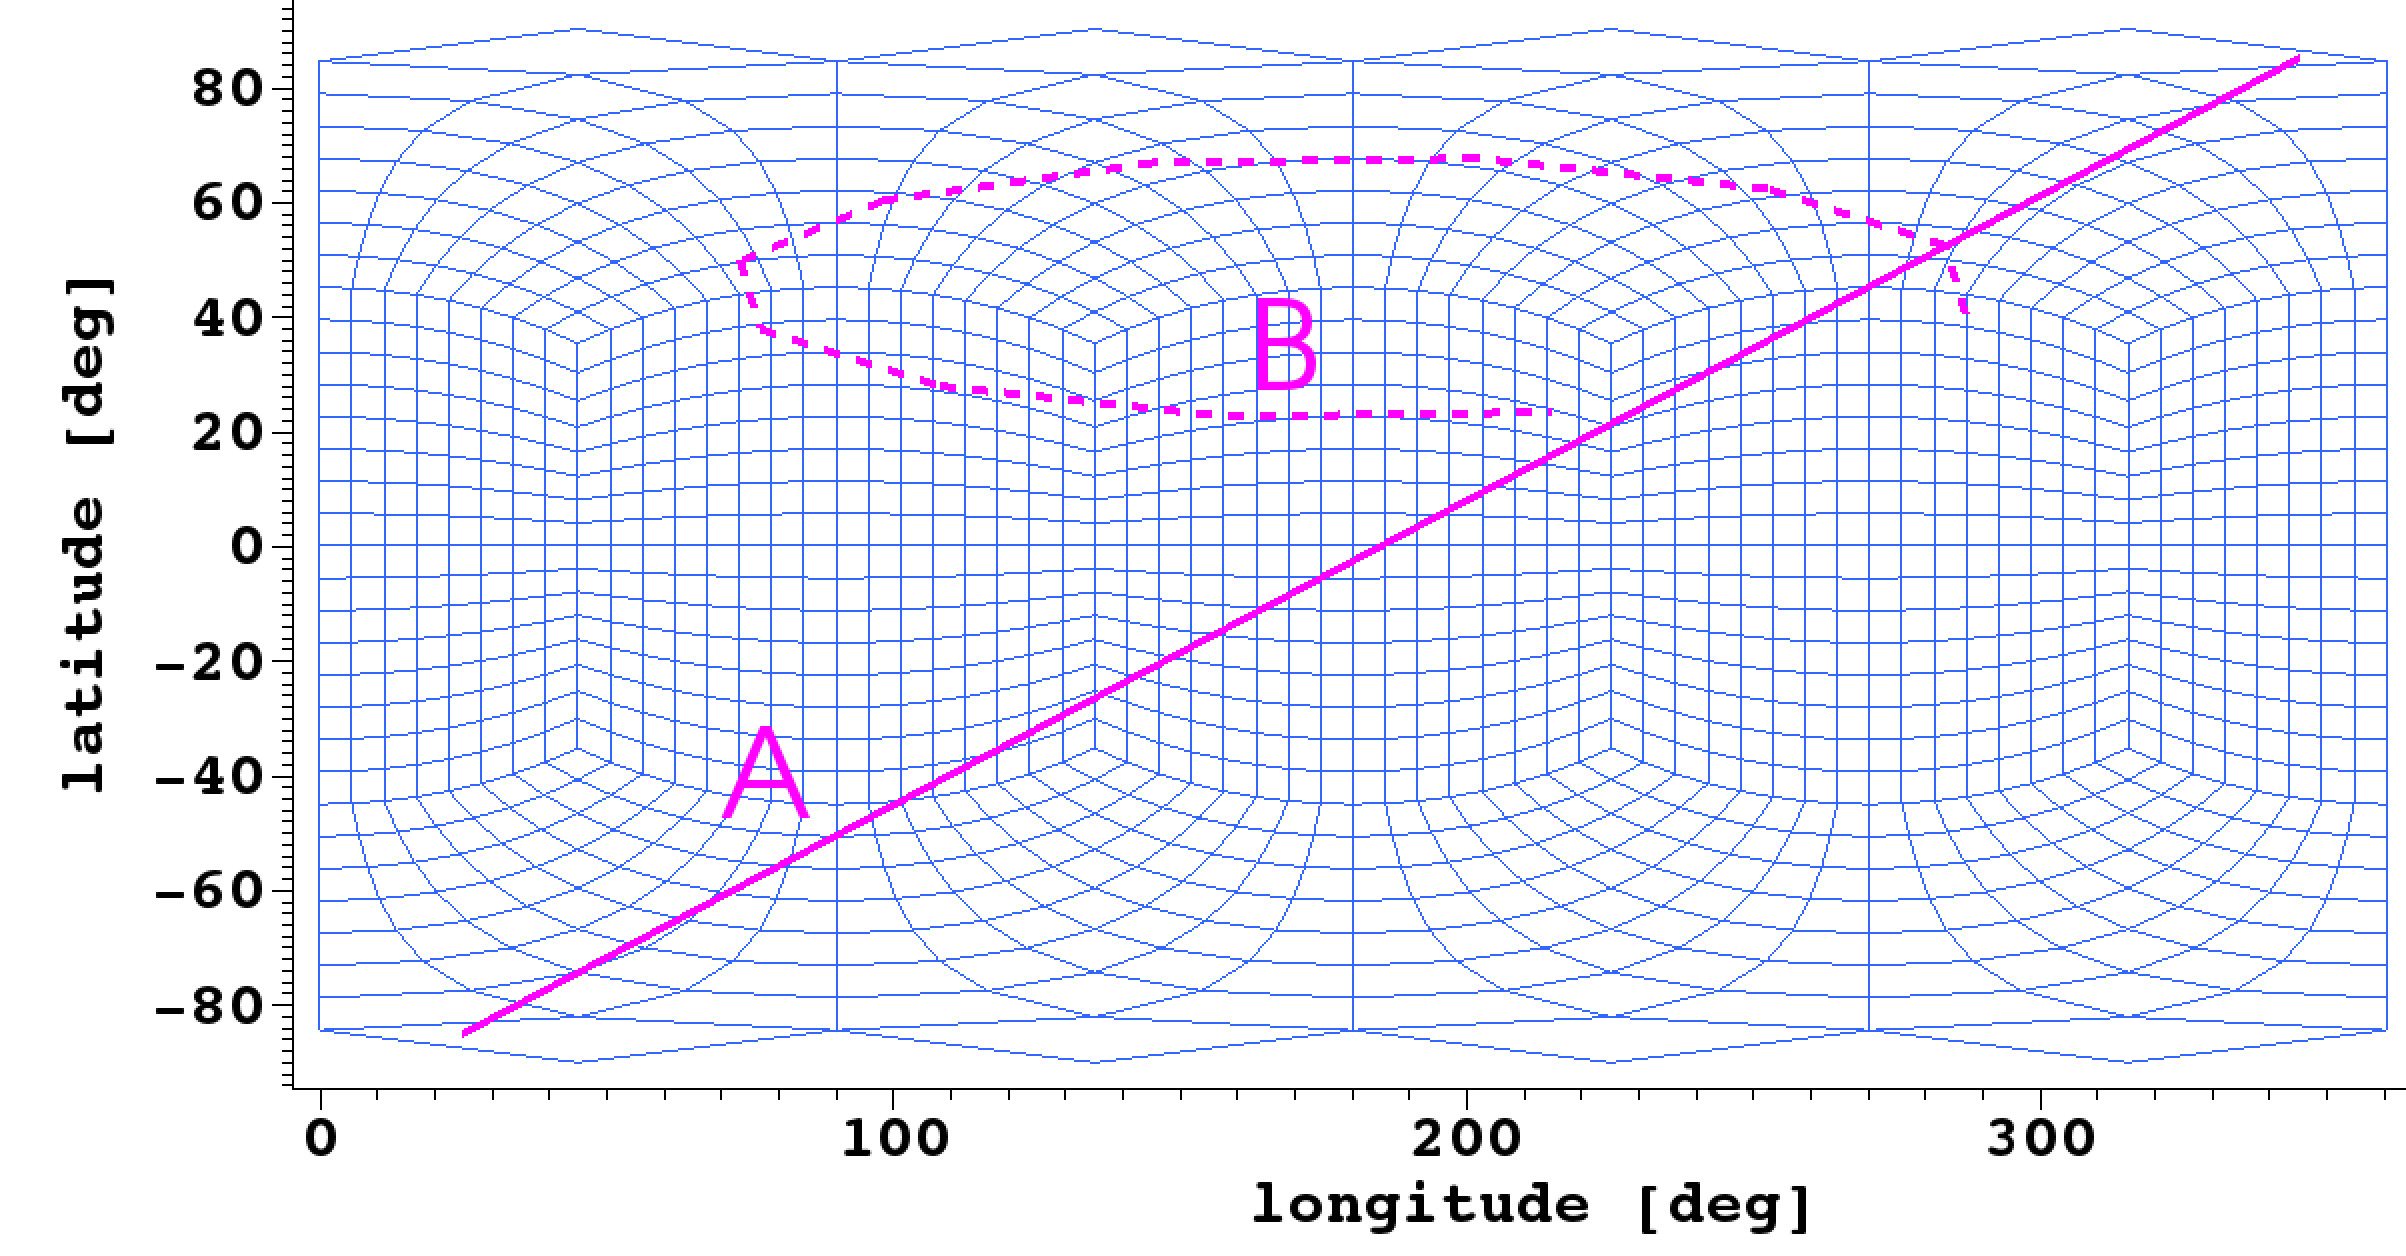
\includegraphics[width=75mm]{fluxOnCubedSphere.png} & 
  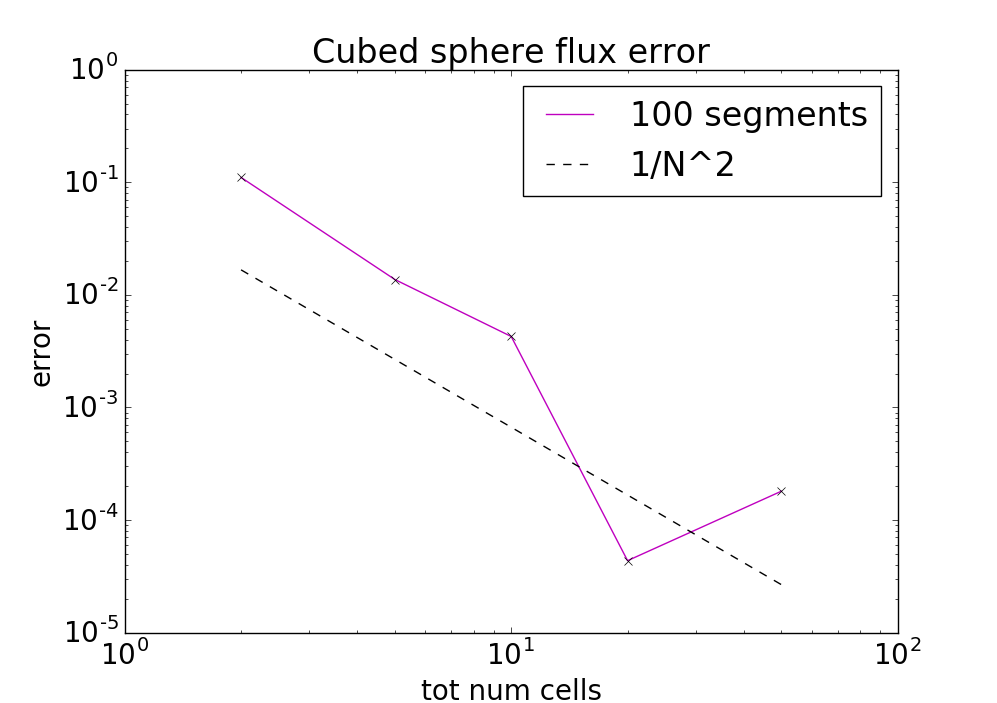
\includegraphics[width=60mm]{cubedSphereFluxError.png} \\
  {Integration path/surface} & {Error is $\sim 1/N^2$} 
  \end{tabular}
\end{frame}

\begin{frame}[t]
  \frametitle{Summary}
    \begin{block}{Type of field $\rightarrow$ discretised field staggering $\rightarrow$ basis functions $\rightarrow$ interpolation method}
      \begin{itemize}%[<+-| alert@+>]
	  \item use bilinear for nodal (scalar) field
	  \item use {\color{red} edge} for vector field - conserves line integrals (e.g. voltage)
	  \item use {\color{red} face} for pseudo-vector field - conserves flux integrals (magnetic flux)
	  \item use cell for pseudo-scalar fields - conserves volume integrals (total mass)
    \end{itemize}
    \end{block}
    \begin{block}{Masking and partially valid cells?}
	 Ok if taking account of partial cell, faces, edges when setting cell, face and edge integrals. Done!
  \end{block}
\end{frame}

\begin{frame}[t]
  \frametitle{Summary (2)}
    \begin{block}{What about tetrahedra?}
      Similar approach except that the basis functions are Whitney's bases (1957)
    \end{block}
    \begin{block}{Higher order basis functions?}
    Initial work indicates that higher order basis functions can be used. These also satisfy the orthogonality condition $\int_i \phi_j = \delta_{ij}$
    on sub-cell edges, faces and cells. Quadratic elements effectively 
     split each cell into 8 sub-cells, each face into 4 sub-faces and each edge into 2 sub-edges. 
  \end{block}
    \begin{block}{The time is ripe to treat interpolation with the same rigour as modelling}
    	``Mimetic Interpolation of Vector Fields on Arakawa C/D Grids'': https://journals.ametsoc.org/doi/10.1175/MWR-D-18-0146.1
  \end{block}
\end{frame}

\end{document} 